\documentclass[11pt, oneside]{article} 
\usepackage{geometry}
\geometry{letterpaper} 
\usepackage{graphicx}
	
\usepackage{amssymb}
\usepackage{amsmath}
\usepackage{parskip}
\usepackage{color}
\usepackage{hyperref}

\graphicspath{{/Users/telliott/Github/calculus_book/png/}}
% \begin{center} 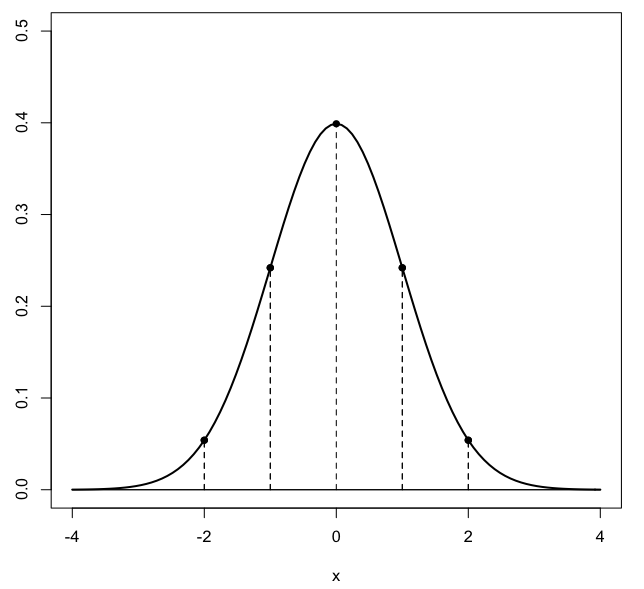
\includegraphics [scale=0.4] {gauss3.png} \end{center}

\title{Primes}
\date{}

\begin{document}
\maketitle
\Large

\subsection*{prime numbers}
As you know, the positive integers $a > 1$ are of two types.  Prime numbers have no factors other than themselves and $1$, while composite numbers have at least one other factor.  If they are not perfect squares they have two.

The first few primes are:
\begin{verbatim}
2 3 5 7 11 13 17 19 23 29 ...
\end{verbatim}

\subsection*{The sieve of Eratosthenes}

Eratosthenes is famous in mathematics for his "sieve" which allows one to compute the prime numbers in an economical fashion.  We took note of him previously in talking about the circumference of the earth.

The sieve is operated by first enumerating all the integers to some upper limit (here $120$).  To do things manually it is convenient to use rows with $10$ values, so there are $12$ rows in all here.  Most of the boxes have not yet been numbered.

Starting with the first prime number, $2$ (red), eliminate all the numbers divisible by $2$ (all the even numbers).  Here this has been done by coloring red all of the squares in the even numbered columns (all numbers ending in $2,4,6,8,0$).

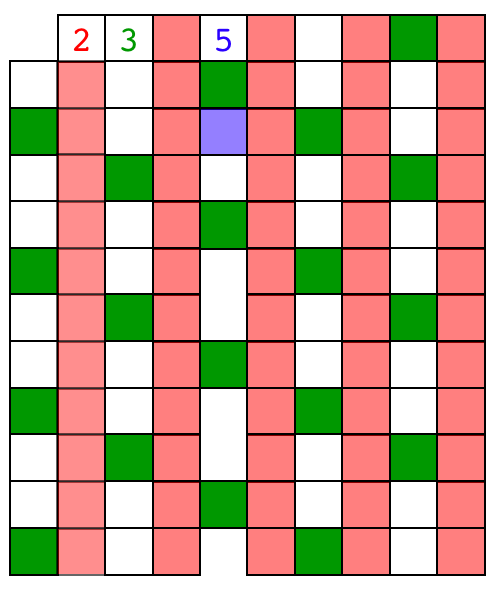
\includegraphics [scale=0.40] {sieve6.png}
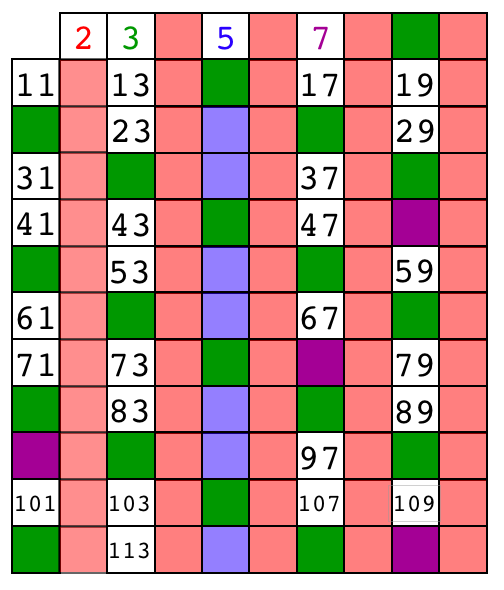
\includegraphics [scale=0.40] {sieve7.png}

Next, do the same thing with $3$ (green).  $6$ was already eliminated previously, but odd multiples of $3$ like $9$ and $15$ go away at this step.

The next larger number that still has a white square is $5$.  The only squares eliminated are the white ones in the fifth row. The first value specifically eliminated at the $5$ step is $25$.  Continue with $7$, eliminating $49, 77, 91$ and $119$.

The sieve ends when the number for the beginning of the next round, the smallest number not yet eliminated, is greater than the square root of the upper limit (here $\sqrt{120}$).  So $7$ is used for the last round, because after that round the smallest remaining integer is $11$, but we terminate since $11^2 = 121 > 120$.

The graphic shows all the numbers which have yet to be eliminated after the round of $7$.   All of these numbers, $11$, $13$, $17$, and so on, as well as those used as divisors for each round of the sieve ($2, 3, 5, 7$), are prime numbers.

By testing for division by $2, 3, 5$ and $7$, we have found the first $30$ prime numbers.

From a performance standpoint, it is important that we do not need to carry out division.  All that is really needed is repeated addition.  Coding this algorithm in, say, Python is a good challenge.  A bigger challenge is to come up with a method to \emph{grow} the list of primes on demand.  This can be done by keeping track of the first value to be tested above the limit, for each prime in the current list.

\subsection*{infinite primes}

Euclid has a proof that the number of primes (the size of the set of primes) is infinite.

The proof is by contradiction:

Suppose the set of primes $P$ is finite, and that $p_1$, $p_2 \dots p_k$ are all of the primes.  Construct the following numbers:
\[ q = (p_1 \times p_2 \times \dots p_k)  \]
\[ r = q + 1 \]
For a prime number $p$ to divide $r$, it must divide the difference between $r$ and $q$.  But that difference is $1$ and so can't be divided evenly by any prime.

Therefore, none of the known primes divides $r$, and $r$ is either a prime not in the set of known primes, or the set was originally incomplete.

In either case, the assumption that the set of primes is finite leads to a contradiction.

$\square$

Even for a relatively small number of primes, the second case may hold.  Consider
\[ (2 \cdot 3 \cdot 5 \cdot 7 \cdot 11 \cdot 13) + 1 = 30031 \]
$30031$ is not prime but is divided by two primes not in the list:  $59$ and $509$.

\subsection*{prime factorization}

We will prove that every integer has a unique prime factorization.  This is also called \emph{the fundamental theorem of arithmetic}.

\[ n = p_1 \cdot p_2 \dots p_n \]

First, we need a preliminary result, which is called \emph{Euclid's lemma}.

Every natural number $n > 1$, i.e. every positive integer greater than $1$, is either prime, or it is the product of two smaller natural numbers $a$ and $b$.

But the same is true of $a$ and $b$ in turn.

Therefore, every number that can be factored into $a$ and $b$ is the product of the prime factors of $a$ times the prime factors of $b$.  

The notation $m|n$ means $m$ divides $n$ (evenly).

Suppose a given prime $p$ divides $n = ab$, i.e. $p|n$.  Then either $p|a$ or  $p|b$ (or both).

\subsection*{Proof of existence}

The proof is by induction.

Assume the lemma is true for all numbers between $1$ and $n$.  

It is certainly true for say, $n \le 100$, because we can check each case.  Start with $n = 101$.

$\circ$ \ If $n$ is prime (as it is here) there is nothing to prove and we move to $n + 1$.  

$\circ$ \  $n$ is not prime, then there exist integers $a$ and $b$ (with $1 < a \le b < n$) such that $n = a \times b$.

$\circ$ \ By the induction hypothesis, since $a < n$ and $b < n$, $a$ has prime factors $p_1 p_2 \dots$ and $b$ has prime factors $q_1 q_2 \dots$ so
\[ n = ab = p_1 p_2 \dots q_1 q_2 \dots \]

This shows that there exists a prime factorization of $n$.

\subsection*{Proof of uniqueness}

To show that the prime factorization is unique suppose that $n$ is the smallest integer for which there exist two different factorizations:
\[ n = p_1 p_2 \dots = q_1 q_2 \dots \]
    
Pick the first factor $p_1$.  Since $p_1$ divides $n = q_1 q_2 \dots$, by Euclid's lemma, it must divide some particular $q_j$.  Rearrange the $q$ so that $q_j$ is first.

But since $p_1$ divides $q_1$ and both are prime, it follows that $p_1 = q_1$. 

Now continue the same process with all the factors $p_i$.

wikipedia:

    This can be done for each of the $m$ $p_i$'s, showing that $m \le n$ and every $p_i$ is some $q_j$. Applying the same argument with the p and q reversed shows $n \le m$ (hence $m = n$) and every $q_j$ is a $p_i$.
    
$\square$
    
\subsection*{elegant proof}

Hardy and Wright (\emph{Theory of Numbers}, sect. 2:11) have a second proof, which is quite delightful.  It is given here almost verbatim:

    Let us call numbers which can be factored into primes in more than one way, \emph{abnormal}, and let $n$ be the smallest abnormal number.

Different factorization:

The same prime $P$ cannot appear in two different factorizations of $n$, for, if it did, $n/P$ would be abnormal and yet $n/P < n$, the smallest abnormal number.

Thus, we have that

\[  = p_1 p_2 \dots = q_1 q_2 \dots \]
    
where the $p$ and $q$ are primes, and no $p$ is a $q$ and no $q$ is a $p$.

If there exist abnormal numbers with two such factorizations, they must be completely different.

\subsection*{the contradiction}

We may take $p_1$ to be the least $p$ (if the least $q$ is less than the least $p$, switch labels on all the $p$'s and $q$'s).  

Since $n$ is composite, $p_1^2 \le n$.

The same is true for $q_1$ and (since $p_1 \ne q_1$), we have that $p_1 q_1 < n$.

Hence, if $N = n - p_1 q_1$, we have $0 < N < n$ and also that $N$ is not abnormal.

Now $p_1 | n$ and since $N = n - p_1 q_1$, so $p_1 | N$.

Similarly $q_1 | N$.  Hence $p_1$ and $q_1$ both appear in the unique factorizations of both $N$ and $p_1 q_1$.

From this it follows that $p_1 q_1 | n$ and hence $q_1 = n/p_1$.  But $n/p_1$ is less than $n$ and has the unique prime factorization $p_2 p_3 \dots$.

Since $q_1$ is not a $p$, this is impossible.  Hence there cannot be any abnormal numbers, and this is the fundamental theorem.

$\square$

\end{document}